\documentclass[border=10pt]{standalone}

\usepackage{ctex}
\usepackage{tikz}
\usetikzlibrary{er,positioning,trees}

\begin{document}
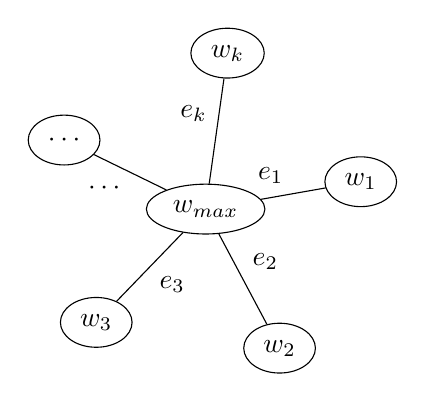
\begin{tikzpicture}[auto,node distance=1.5cm]
	\node[attribute] {$w_{max}$}
	[clockwise from=10,level distance=2cm,sibling angle=72]
	child {
		node[attribute] {$w_1$}
		edge from parent node {$e_1$}
	}
	child {
		node[attribute] {$w_2$}
		edge from parent node {$e_2$}
	}
	child {
		node[attribute] {$w_3$}
		edge from parent node {$e_3$}
	}
	child {
		node[attribute] {$\cdots$}
		edge from parent node {$\cdots$}
	}
	child {
		node[attribute] {$w_k$}
		edge from parent node {$e_k$}
	};
\end{tikzpicture}

\end{document}
